\documentclass[a4paper,12pt]{article}

%% Language and font encodings
\usepackage[italian]{babel}
\usepackage[utf8x]{inputenc}
\usepackage[T1]{fontenc}

%% Sets page size and margins
\usepackage[a4paper,top=2cm,bottom=2cm,left=3cm,right=3cm,marginparwidth=1.75cm]{geometry}

%% Useful packages
\usepackage{graphicx}
\usepackage{bigstrut}
\usepackage{hyperref}
\usepackage[figurename=Figura]{caption}
\usepackage[tablename=Tabella]{caption}
\hypersetup{colorlinks=true, urlcolor=blue, linkcolor=black}
\title{Alberi di Decisione per Intrusion Detection}
\author{Lorenzo Pesci}

\begin{document}
\maketitle

\section{Introduzione}
Lo scopo di questo elaborato è quello di utilizzare diverse implementazioni di \textit{Decision Trees} relativamente al problema dell'Intrusion Detection.

\
\begin{figure}[h]
    \centering
    \captionsetup{justification=centering, margin=1cm}
    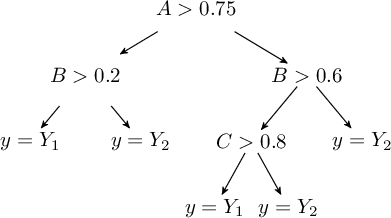
\includegraphics[width=0.6\textwidth]{./fig_decisiontree}
    \vspace*{5mm}
    \caption{Un esempio di albero di decisione. [\textit{ce.unipr.it}]}
    \label{fig:dec}
\end{figure}

\subsection{Alberi di Decisione}

Nell’ambito del \textit{Machine Learning} un metodo semplice ed efficace per risolvere problemi di classificazione è quello di utilizzare gli alberi di decisione.
\newline

Un albero di decisione, costruito a partire da un insieme di dati iniziali (\textbf{dataset}), è un albero in cui ogni nodo interno è associato ad una particolare “domanda” su una certa caratteristica dei dati. Da questo nodo escono tanti archi quanti sono i possibili valori che la caratteristica può assumere, fino a raggiungere le foglie che indicano la categoria associata alla decisione.
\newline

Lo scopo è quello di allenare questo albero su alcuni esempi di dati (\textit{training set}) in modo da poter classificare altri dati non precedentemente visionati (\textit{test set}) con un certo livello di confidenza.
\newline

Un problema comune con gli alberi di decisione è che spesso si adattano fin troppo bene ad alcune
	caratteristiche specifiche solo del \textit{training set}, e questo porta ad un calo delle
	prestazioni sul \textit{test set}.  

\subsection{Intrusion Detection}
L'Intrusion Detection è un sistema che viene utilizzato per rilevare e contrastare gli attacchi
	informatici che avvengono in un sistema o in una determinata rete. Generalmente un intruso è
	definito come un sistema, un programma o una persona che tenta di entrare in un sistema di
	informazione o eseguire un'azione non legalmente consentita. 
\newline
In particolare in questo esercizio ci concentreremo su quattro tipologie di attacchi:
\newline \textit{\textbf{-Denial of Service Attacks (DoS)}}: è un tipo di attacco in cui l'hacker rende le risorse di calcolo o di memoria troppo occupate o troppo piene per servire legittime richieste di rete e quindi negare agli utenti l'accesso a una macchina. (es. apache)
\newline \textit{\textbf{-Remote to User Attacks (R2L)}}: un attacco da remoto a utente è un attacco in cui un utente invia pacchetti a una macchina su Internet, a cui non ha accesso per esporre le vulnerabilità delle macchine e i privilegi di exploit che un utente locale avrebbe sul computer. (es. xlock)
\newline \textit{\textbf{-User to Root Attacks (U2R)}}: sono exploit in cui l'hacker si avvia sul sistema con un normale account utente e tenta di sfruttare le vulnerabilità nel sistema per ottenere privilegi di super utente.  (es. perl)
\newline \textit{\textbf{-Probing}}: è un attacco in cui l'hacker esegue la scansione di una macchina o di un dispositivo di rete al fine di determinare punti deboli o vulnerabilità che potrebbero essere sfruttati in seguito per compromettere il sistema. Questa tecnica è comunemente usata nel data mining. (es. portsweep)

\section{Esperimento}
L'esperimento è stato condotto utilizzando il data set della \href{http://kdd.ics.uci.edu/databases/kddcup99/kddcup99.html}{KDD Cup 1999}.
	 Questo set di dati è stato fornito dal MIT Lincoln in collaborazione con l'Air Force Lan ed
	 è utile per verificare e utilizzare il classificatore di sistema.
\newline

Questo è il set di dati utilizzato per la terza competizione internazionale di scoperta della conoscenza e strumenti di data mining, che si è svolta in concomitanza con la KDD-99. La quinta conferenza internazionale sulla scoperta della conoscenza e il data mining. L'obiettivo della competizione era costruire un rilevatore di intrusione di rete, un modello predittivo in grado di distinguere tra connessioni "cattive", chiamate intrusioni o attacchi e connessioni "buone" normali. Questo database contiene un set standard di dati da verificare, che include un'ampia varietà di intrusioni simulate in un ambiente di rete militare.
\newline

L'obiettivo dell'esperimento è quello di riprodurre con maggior accuratezza possibili le tabelle 2 e 3 proposte in \href{https://www.semanticscholar.org/paper/Naive-Bayes-vs-decision-trees-in-intrusion-systems-Amor-Benferhat/16a778c5d83cce2f4c4af46efafb927e7d0d8e60}{(Amor et al.2004)}.
\
\begin{figure}[h]
    \centering
    \captionsetup{justification=centering, margin=1cm}
    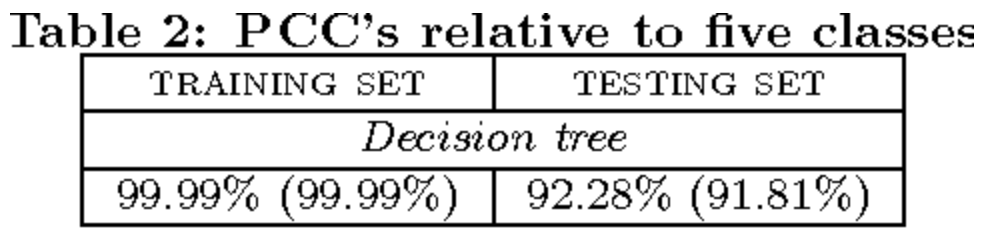
\includegraphics[width=0.6\textwidth]{./Table2}
    \vspace*{5mm}
    \caption{Tabella 2 (Amor et al. 2004)}
    \label{fig:dec}
\end{figure}
\newline
\begin{figure}[h]
    \centering
    \captionsetup{justification=centering, margin=1cm}
    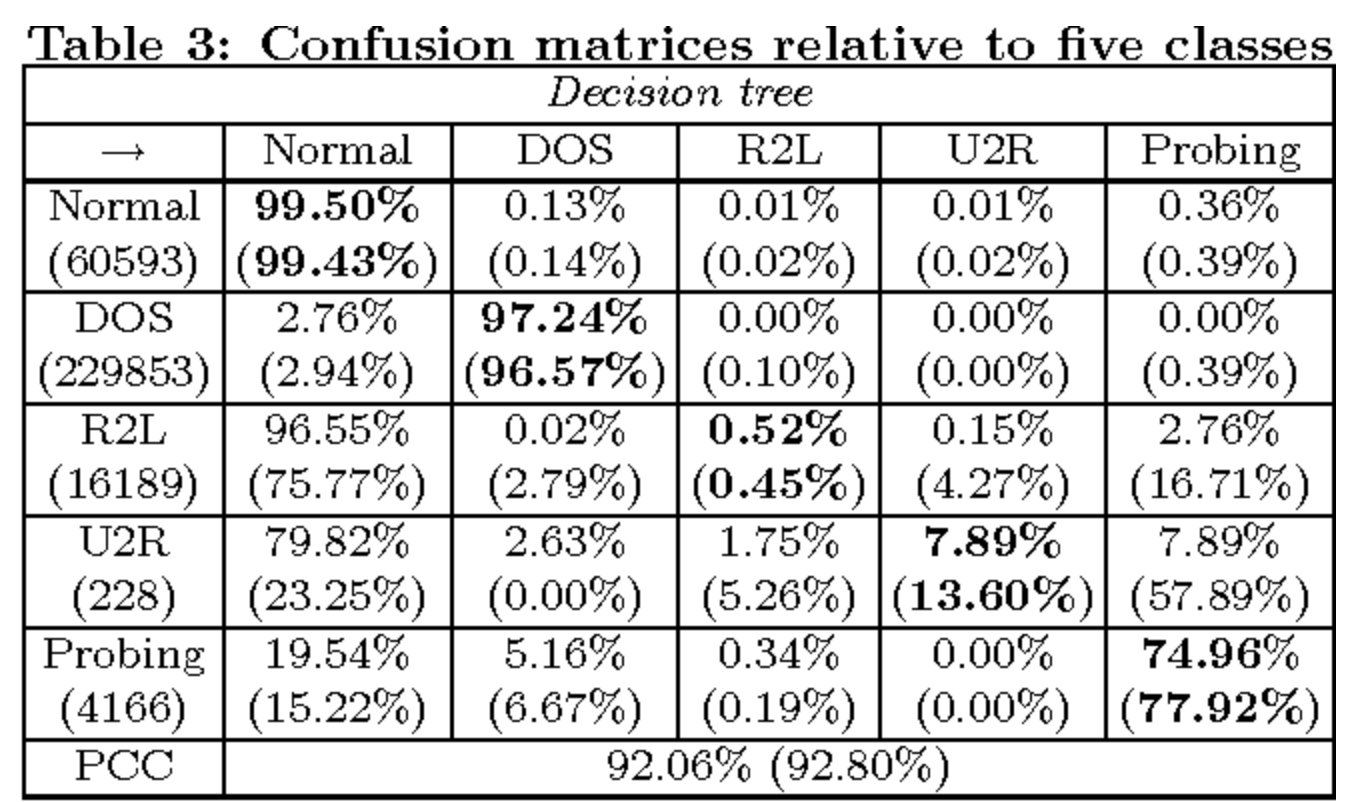
\includegraphics[width=0.6\textwidth]{./Table3}
    \vspace*{5mm}
    \caption{Tabella 3 (Amor et al. 2004)}
    \label{fig:dec}
\end{figure}
\newline

\section{Implementazione}
Il progetto è stato sviluppato con Python versione 3.7 e richiede l'installazione delle librerie
\textit{pandas} e \textit{sklearn}.

\subsection{preprocessing.py}
Nel file \textit{preprocessing.py} vengono mappate tutte le possibili tipologie di attacchi con l'intero corrispondente. In particolare \textit{Normal Attack = 0}, \textit{DOS Attack = 1}, \textit{R2L Attack = 2}, \textit{U2R Attack = 3} e \textit{Probing = 4}.
\newline

Inoltre poichè gli algoritmi di costruzione di un albero di decisione classificano correttamente gli esempi del training set, a condizione che nel training set non siano presenti dati rumorosi. Per far fronte a questa problematica è stata applicata la codifica \textbf{\textit{one hot}} alle variabili categoriche corrispondenti alle colonne \textit{flag}, \textit{protocol\_type} e \textit{service}, in modo da ridurre il rumore dei dati.

\subsection{dt\_predict.py} 
Nel file \textit{dt\_predict} vengono effettuate le predizioni sui dati. 
\newline
Viene utilizzato \textit{DecisionTreeClassifier}, preso dalla libreria \textit{sklearn} che contiene il classificatore basato sugli alberi di decisione. Come criterio di decisione è stato usato \textit{entropy}, come splitter è stato usato \textit{random}. Inoltre è stata fissata la massima profondità raggiungibile dall'albero (max\_depth=15) e  il numero minimo di campioni richiesti in una foglia (min\_samples\_leaf=6). Questi parametri sono stati scelti in base ai parametri contenuti nella pagina \href{http://citeseerx.ist.psu.edu/viewdoc/download?doi=10.1.1.122.5800&rep=rep1&type=pdf}{Data Mining Techniques for Intrusion Detection}.

\subsection{data\_names.py} 
Nel file \textit{data\_names} sono presenti due liste, una contenente i features names e l'altra contente gli attribute names.

\subsection{Test}
Sono stati effettuati numerosi test, utilizzando le due diverse tipologie di criteri per gli alberi di decisione, \textit{entropy} e \textit{gini}, le due diverse tipologie di split,  \textit{best} e \textit{random}. Sono stati inoltre modificati gli interi assegnati a \textit{max\_depth} e \textit{min\_samples\_leaf}, avendo cura di combinare tutte le possibilità. 

\section{Risultati}
Di seguito è riportato il miglior risultato ottenuto dai vari test: 
\
\begin{figure}[h]
    \centering
    \captionsetup{justification=centering, margin=1cm}
    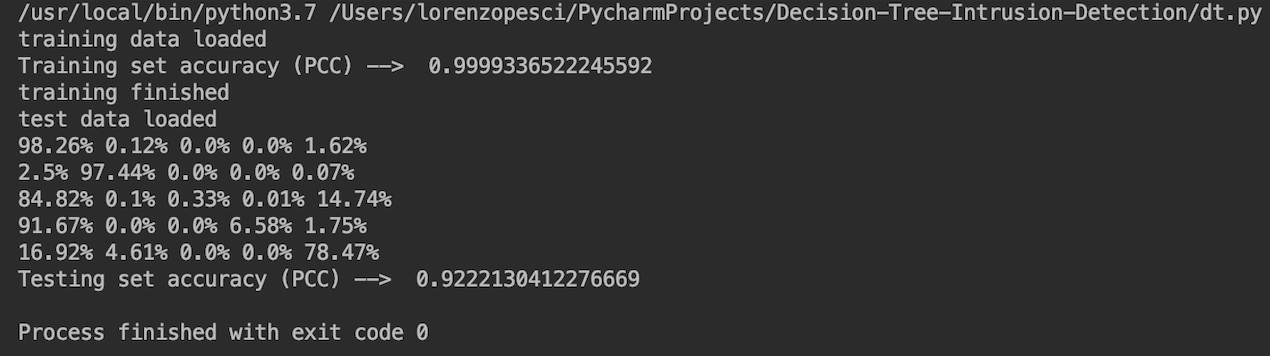
\includegraphics[width=0.6\textwidth]{./bestresult}
    \vspace*{5mm}
    \caption{Miglior test effettuato}
    \label{fig:dec}
\end{figure}
\newline

Riportiamo i dati ottenuti in due distinte tabelle:

\begin{center}
\vspace*{0.1cm}
\begin{tabular}{|c|c|}
\hline
\textbf{TRAINING SET}\bigstrut & \textbf{TESTING SET}\\\hline
99.99\% & 92.22\%\\\hline

\end{tabular}
\captionsetup{justification=centering}
\captionof{table}{Dati della Figura 4, riportati in un grafico.}
\label{tab:tab1}
\end{center}


\begin{center}
\vspace*{0.5cm}
\begin{tabular}{|c|c|c|c|c|c|}
\hline
$\longrightarrow$ & \textbf{Normal}\bigstrut & \textbf{DOS} & \textbf{R2L} & \textbf{U2R} & \textbf{Probing} \\\hline
\textbf{Normal}\bigstrut & \textbf{98.26\%} & 0.12\% & 0.0\% & 0.0\% & 1.62\%\\\hline
\textbf{DOS}\bigstrut & 2.5\% & \textbf{97.44\%} & 0.0\% & 0.0\% & 0.07\%\\\hline
\textbf{R2L}\bigstrut & 84.82\% & 0.1\% & \textbf{0.33\%} & 0.01\% & 14.74\%\\\hline
\textbf{U2R}\bigstrut & 91.67\% & 0.0\% & 0.0\% & \textbf{6.58\%} & 1.75\%\\\hline
\textbf{R2L}\bigstrut & 16.92\% & 4.61\% & 0.0\% & 0.0\% & \textbf{78.47\%}\\\hline
\end{tabular}
\captionsetup{justification=centering}
\captionof{table}{Dati della Figura 4, riportati in un grafico.}
\label{tab:tab1}
\end{center}

\section{Conclusione} 
Dall'analisi del set di dati della \href{http://kdd.ics.uci.edu/databases/kddcup99/kddcup99.html}{KDD Cup 1999}, è apparso evidente che erano necessari rivelatori specializzati per classificare i vari tipi di attacchi informatici che avvengono in un sistema o in una rete. Gli attacchi di tipo DoS o Probing si sono dimostrati molto facili da classificare utilizzando modelli semplici. Invece gli attacchi più rari come R2L e U2R necessitano di rivelatori più sofisticati.


\end{document} 